% !TeX spellcheck = en_GB

\section{Problem 1}

In what follows, I present the implementation of the \textbf{streaming algorithms} we studied in class to estimate some useful statistics on data streams. You can find the source code in the material attached with this documentation.\medskip

\noindent\textbf{Disclaimer}: to run my code, be sure to be on a Linux machine (or any other that allows you to run Bash scripts) and have Python 2.7 installed. Note that some additional Python modules are required (see following sections).


\subsection{Flajolet-Martin algorithm}

Let $X = (x_1, x_2, \ldots, x_m)$ be a sequence (stream) of elements where $x_j \in \{1,\ldots,n\}$ and $m_i = |\ \{j \ | \ x_j = i\}\ |$ be the number of occurrences of $i \in \{1,\ldots,n\}$ in $X$.
The $k\text{-}th$ \textbf{frequency moment} of $X$ is defined as
\begin{align}
	F_k = \sum_{i = 1}^{n} m_{i}^k \label{fk}
\end{align}
From (\ref{fk}), we can trivially deduce that $F_0$ is equal to the number of distinct elements in the stream. \textbf{Flajolet-Martin}\cite{fm} algorithm is a scheme for approximating $F_0$ with a single pass, and a space complexity which is \textbf{logarithmic} in the maximum number of distinct elements.\\
The idea behind the algorithm is to exploit some particular properties of \textbf{hash signatures}. In particular, we want to consider a \textbf{binary} signature for each element in the stream and look at how many 0's it ends in, i.e. the so-called \textbf{tail length}. Given an hash function $h$, let $R$ be the \textbf{maximum} tail length seen so far in the stream. Then, we can estimate $F_0$ computing the value $2^R$ (see \cite{mmd}, section 4.4.2 for further details).\\
To improve the \textbf{accuracy} of the approximation, we could combine a bunch of independent estimates, obtained using several different (random) hash functions. However, there exist some issue to take into account when combining these results. Indeed, increasing the value of $R$ by 1 corresponds to double the value of $2^R$. For instance, a single occasional outsized value of $2^R$ could hugely affect the \textbf{average}, with a corresponding loss of accuracy. Also taking the \textbf{median} of the independent estimates is not effective, since it would always be a power of 2, thus, it could be impossible to obtain a close estimate. An effective workaround is to combine the two methods:
\begin{enumerate}
	\item group independent estimates into smaller \textbf{sub-groups} and compute the \textbf{average} of each.
	
	\item compute the \textbf{median of the averages}.
\end{enumerate}
This trick allows to reduce the influence of the issues described above and to obtain a close approximation for the $0\text{-}th$ frequency moment.


\subsection{Alon-Matias-Szegedy algorithm}

Alon-Matias-Szegedy algorithm is a scheme for approximating the $2\text{-}nd$ frequency moment of a stream ($F_2$), that is considered an \textbf{index of homogeneity}, with a single pass, and a space complexity which is \textbf{logarithmic} in the maximum number of distinct elements and the size of the stream.\\
Let $\{1,\ldots,n\}$ be the set of distinct elements in the stream. The algorithm consists in \textbf{hashing} each $i \in \{1,\ldots,n\}$ to a random element $\epsilon_i \in \{-1,+1\}$ and maintaining the sketch
\begin{align*}
	Z = \sum_{i} \epsilon_i m_i
\end{align*}
Then, we can take $X = Z^2$ as an approximation of $F_2$. To improve the \textbf{accuracy} of the approximation, we could take the \textbf{average} of a bunch of independent estimates, obtained using several different (random) hash functions (used to map elements to $\{-1,+1\}$). Indeed, we have that \textbf{on expectation} this value is equal to the $2\text{-}nd$ frequency moment (see \cite{mmd} (section 4.5) and \cite{dm-streams} for further details and formal proof).


\subsection{Implementation}

I created a Python module (named \textit{freq\_moments\_estimation.py}) that encapsulates the algorithms described above. In particular, both of them are implement in an \textbf{online} fashion, such that as soon as a new element of the stream arrives it is possible to update the estimates and get the approximation.\\
To check the validity of my implementations, I made a Bash script that computes frequency moments \textbf{exactly}, dropping the streaming model and given that the input consists in a single \textit{.txt} file. In particular, I used a combination of \textit{sort} and \textit{uniq} commands to get elements frequencies and then applied definition (\ref{fk}) for $k = 0$ and $k = 2$. To run the script, open a terminal and type
\begin{lstlisting}
$ ./compute-freq-moments.sh -s file.txt
\end{lstlisting}
where \textit{file.txt} is the file containing the stream (one element per line).\\ 
\textbf{Note}: executing script with "-s" option \textbf{at least once} is required to reuse results when evaluating the accuracy of streaming algorithms (see later).\\

\noindent For the first test, I used the provided NASA access log dataset\cite{nasa}. First of all, I made a simple Python script to pre-process the dataset, to retain only the info about IP addresses. To run the script, open a terminal and type
\begin{lstlisting}
$ python preprocess_access_log.py
\end{lstlisting}
The corresponding output will be stored into a file named \textit{access\_log\_prep.txt}, that can be used as input for the Bash script to generate a file named \textit{access\_log\_prep\_results.txt}, containing the \textbf{exact values} of the frequency moments.
Thus, we can perform the estimates for that values, running a Python script named \textit{estimate\_access\_log\_freq\_moments.py}. Before running, open the file and set the number of \textbf{independent estimates} and the number of \textbf{estimates per group} to be used. Then, open a terminal and type
\begin{lstlisting}
$ python estimate_access_log_freq_moments.py
\end{lstlisting}
The output of this script consists in the estimates for $0\text{-}th$ and $2\text{-}nd$ frequency moments and the absolute and relative errors (with respect to actual values).\\

\noindent For the second test, I generated a stream consisting of messages taken from Twitter. To do that, I used \textit{tweepy}\cite{tweepy}, an easy-to-use and open source Python wrapper for \textbf{Twitter Streaming API}\cite{twitter}. The source code for this test is located in a Python script named \textit{generate\_tweets\_stream.py}. Note that to run the script Twitter \textbf{API keys} are required (in \textit{twitter\_secret\_keys\_template.txt} there are instructions to add them to the source code). See \cite{twitter} to know how to generate API keys. Then, open a terminal and type
\begin{lstlisting}
$ python generate_tweets_stream.py
\end{lstlisting}
Then program will output to screen the tweets that matches the given query (that can be easily adjusted in the script) and the values of frequency moments estimates (according to the parameters set in the code) as soon as a new one arrives.
In addition, all tweets will be stored into a file named \textit{tweets.txt}. This output can be used as input for the Bash script to generate a file named \textit{tweets\_results.txt}, containing the \textbf{exact values} of the frequency moments.
Thus, we can perform the estimates for that values, running a Python script named \textit{estimate\_tweets\_freq\_moments.py}. Similarly to the previous test, we can set the parameters to be used and then open a terminal and type
\begin{lstlisting}
$ python estimate_tweets_freq_moments.py
\end{lstlisting}
The output will be of the same kind of the one obtained in the previous test.


\subsection{Results}

In what follows, I report some results obtained from several different run of the estimates scripts.

\begin{center}
	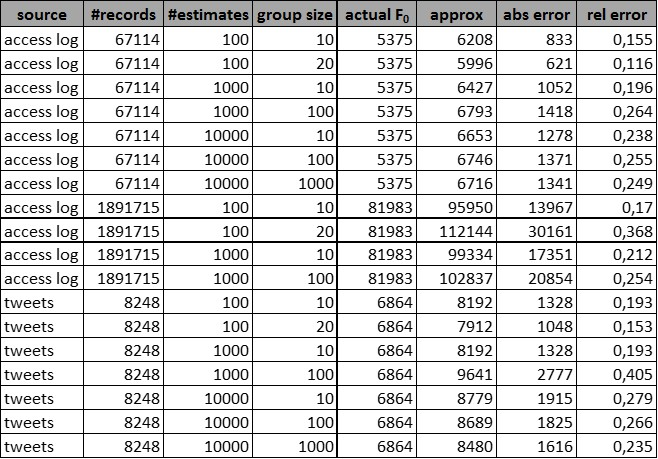
\includegraphics[scale=0.7,]{img/f0.jpg}
\end{center}

\bigskip
\begin{center}
	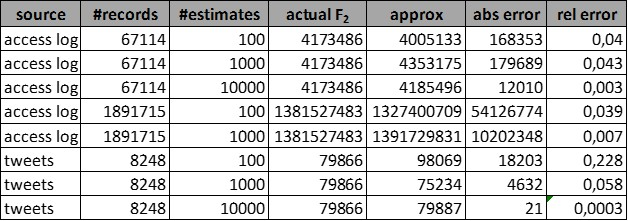
\includegraphics[scale=0.7]{img/f2.jpg}
\end{center}
